\documentclass{amsart}[12pt]
\usepackage{amsmath, amsfonts, tikz, natbib, array}
\oddsidemargin=0in \evensidemargin=0in
\textwidth=6.6in \textheight=8.7in

\title{Mappings between Euclidean and spherical polygons}
\author{B R S Recht}
\date{December 2018}

\begin{document}

\maketitle

Yadda yadda\cite{kahn}

In the geodesic dome world, geometry is usually synthetic rather than
analytic. That is, geometric constructions are usually expressed in terms of
step-by-step geometric constructions rather than in equations and numeric
values. See, for instance, \cite{kenner}. Implementing a synthetic geometric
construction on a computer can be a pain; analytic specifications are more
amenable to programming idioms.

\section{Definitions}
Unless otherwise specified, the vertices of any given polygon are ordered in
countclockwise order.

\subsection{Spherical geometry}
There are a number of ways to numerically specify points on a sphere. By far
the most common is by latitude and longitude, which appear on every modern map
of the Earth and probably some other planets. Latitude and longitude are
familiar and convenient, but performing extended geometry calculations using
latitude and longitude is a complicated task.

Doing spherical geometry using a 3-component unit vector is more convenient
in a number of ways: the equations are often simpler, and there are no
singularities at the poles. A unit sphere can be defined as the set of all unit
vectors in 3-space; i.e., vectors $\mathbf v = [v_x, v_y, v_z]$ such that the
vector norm $\|\mathbf v \|=1$. Unit vectors are often denoted using a hat:
$\hat{\mathbf v}$. We'll often find ourselves normalizing vectors,
so we may supress the denominator with an ellipsis like so:
\begin{equation}
  \hat{\mathbf v} = \frac{\mathbf{some+really+long+statement}}{\|\dots\|}
\end{equation}
If a vector is an intermediate step to a normalized vector,
we may call it pre-normalized and denote it ${\mathbf v}^*$,
such that $\hat{\mathbf v} = \frac{{\mathbf v}^*}{ \|{\mathbf v}^*\|}$

The shortest distance between two points in Euclidean space is a straight line.
On the sphere, the shortest distance is an arc of the great circle between those
points. The great circle is the intersection of the sphere and a plane passing
through the origin. A plane through the origin can be specified as
$\hat{\mathbf n} \cdot \mathbf v = 0$, where $\hat{\mathbf n}$ is a unit vector
normal to the plane; this vector $\hat{\mathbf n}$ can be used to specify a
great circle. Given two points $\mathbf{\hat{v}_1, \hat{v}_2}$ on the sphere,
the $\hat{\mathbf n}$ of the great circle between those two points is (up to
normalization) their cross product:
\begin{equation}
  \mathbf{\hat{n}} =
\frac{\mathbf{\hat{v}}_1 \times \mathbf{\hat{v}}_2}{\|\dots\|}
\end{equation}

Small circles are the intersection of the sphere with a plane not through
the origin. All planes may be specified in Hessian normal form as
$\mathbf{\hat{n}} \cdot \mathbf v = r$, where $r$ is the minimum distance
between the plane and the origin. The intersection of the plane with the sphere
is determined by $r$ as so:

\begin{itemize}
  \item $r = 0$: Great circle
  \item $r \in (0,1)$: Small circle
  \item $r = 1$: Point
  \item $r > 1$: None
\end{itemize}

The following subsections give some formulas for measurements and constructions
in Euclidean space and on the sphere. Since a sphere is locally Euclidean, the
spherical formulas approach the Euclidean formulas when the measures are small.
Note that some spherical formulas require normalized vectors,
denoted by the hat $\mathbf{\hat{v}}$.

\subsubsection{Distance}
In Euclidean space, the distance between two vertices $\mathbf v_1$ and
$\mathbf v_2$ is given by the usual metric. On the sphere, distance is the
central angle $\theta$, which is given by many equivalent forms: the most
numerically stable one is the one using $\arctan$ given below.
\begin{equation}\begin{split}
\eta & = \|\mathbf v_1-\mathbf v_2\| \\
\theta & = \arctan\left(
  \frac{\|\mathbf{\hat{v}}_1 \times \mathbf{\hat{v}}_2\|}
  {\mathbf{\hat{v}}_1 \cdot \mathbf{\hat{v}}_2}\right)
\end{split}\end{equation}

\subsubsection{Angle}
The angle on a surface at the vertex $v_1$ between $v_2$ and $v_3$ is a
standard expression for Euclidean space. For spheres, it is the dihedral angle
between the planes defined from $v_1$ to $v_2$ and from $v_1$ to $v_3$.
\begin{equation}
  \cos\phi_1 = \mathbf{\hat{c}}_{12} \cdot \mathbf{\hat{c}}_{13}
\end{equation}
where $\mathbf{\hat{c}}_{ij} = \frac{\mathbf{v}_i - \mathbf{v}_j}{\|\dots\|}$
for Euclidean space and $\mathbf{\hat{c}}_{ij} = \frac{\mathbf{\hat{v}}_i
\times \mathbf{\hat{v}}_j}{\|\dots\|}$ for spheres. (This formula also has
equivalent forms using $\sin$ and $\tan$.)

\subsubsection{Area}
The area of an arbitrary polygon with vertices $v_i$ is given by the shoelace
formula. $n$ is the number of vertices in the polygon and
$i = 0 \dots n-1$ is an index for each vertex. $i$ should be treated as if it's
mod $n$, so that it loops around. This formula will give a result for skew
polygons, but the areas of skew polygons are not well-defined.
\begin{equation}
A = \frac{1}{2} \| \sum \mathbf v_i\times \mathbf v_{i+1} \|
\end{equation}
The area of a spherical triangle is the solid angle $\Omega$,
and given by a more elaborate formula. \cite{oosterom}\cite{eriksson}
\begin{equation}
\tan(\Omega/2) = \frac{|\mathbf{\hat{v}_1} \cdot
       \mathbf{\hat{v}}_2 \times \mathbf{\hat{v}}_3|}
       {1+\mathbf{\hat{v}}_1\cdot \mathbf{\hat{v}}_2+\mathbf{\hat{v}}_2
       \cdot \mathbf{\hat{v}}_3+\mathbf{\hat{v}}_3\cdot \mathbf{\hat{v}}_1}
\end{equation}

\subsubsection{Means}
When $n=2$ this formula gives the midpoint between $\mathbf v_1$ and
$\mathbf v_2$. When $n=3$ it gives the centroid of the triangle with
vertices $\mathbf v_1, \mathbf v_2$ and $\mathbf v_3$.
\begin{equation}\begin{split}
\mathbf v_\mu & = \frac{\sum\mathbf v_i}{n} \\
\mathbf{\hat{v}}_\mu & = \frac{\sum\mathbf{\hat{v}}_i}{\|\dots\|}
\end{split}\end{equation}
\subsubsection{Interpolation}
Interpolation in Euclidean space is standard linear interpolation. On the
sphere, interpolation is given by spherical linear interpolation, or slerp.
\begin{equation}
\mathrm{Lerp}(\mathbf{v_1}, \mathbf{v_2}; t) =
       (1-t) \mathbf{v_1} + t \mathbf{v_2}
\end{equation}
\begin{equation}
\mathrm{Slerp}(\mathbf{\hat{v}_1}, \mathbf{\hat{v}_2}; t) =
\begin{cases}\mathbf{\hat{v}_1}
  & \text{if } \mathbf{\hat{v}_1} = \mathbf{\hat{v}_2}\\
        \frac{\sin ((1-t)w)}{\sin (w)} \mathbf{\hat{v}_1} +
       \frac{\sin (tw)}{\sin (w)} \mathbf{\hat{v}_2}
  &\text{otherwise}
      \end{cases}
\end{equation}
where $w = \arccos \mathbf{\hat{v}_1} \cdot \mathbf{\hat{v}_2}$.

\subsubsection{Face normal}
For the purposes of this text, we define the normal to a (Euclidean) polygon as
so, where $n$ is the number of vertices in the polygon and
$i = 0 \dots n-1$ is an index for each vertex:
\begin{equation}
  \hat{\mathbf{n}} =
  \frac{\sum^{n-1}_i \mathbf{v}_i \times \mathbf{v}_{i+1}}{\|\dots\|}
\end{equation}
$i$ should be treated as if it's mod $n$, so that it loops around.
(Note the similarity to the shoelace formula.)
This definition allows for a somewhat sensible extension to skew polygons:
the normal points in a generally reasonable direction for skew polygons.
The normal will be outward-facing if the points are ordered counterclockwise,
and inward-facing if the points are ordered clockwise.

\subsubsection{Skewness}
There's no standard measure of polygon skewness, so this text uses an ad-hoc
measure that seems to work well. This program measures the skewness of a polygon
with 4 or more vertices by this method: Let $\mathbf x_i = \mathbf{v}_i -
\bar{\mathbf{v}}$, where $\bar{\mathbf{v}}$ is the (Euclidean) average of the
points. Calculate the SVD decomposition of the matrix that has $\mathbf x_i$
as rows (or columns). We only need the singular values: since we're in 3d
space, there will be 3 singular values. The \textit{skewness} is the smallest
singular value divided by the sum of the  other two singular values.
If the polygon is flat, the skewness is 0.

\subsection{Triangle and quadrilateral coordinates}

\begin{figure}%[!htbp]
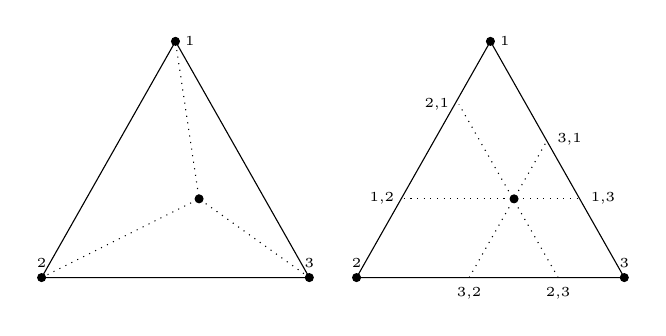
\begin{tikzpicture}
  \draw (0, 0) -- (1.7,3) -- (3.4, 0) -- (0, 0) ;
  \draw[fill] (1.7, 3) circle [radius=0.05] node[anchor=west] {\tiny 1};
  \draw[fill] (0, 0) circle [radius=0.05] node[anchor=south] {\tiny 2};
  \draw[fill] (3.4, 0) circle [radius=0.05] node[anchor=south] {\tiny 3};
  \draw[fill] (2, 1) circle [radius=0.05];
  \draw[dotted] (0,0) -- (2,1) -- (1.7,3);
  \draw[dotted] (3.4, 0) -- (2,1);

  \draw (4, 0) -- (5.7,3) -- (7.4, 0) -- (4, 0) ;
  \draw[fill] (5.7, 3) circle [radius=0.05] node[anchor=west] {\tiny 1};
  \draw[fill] (4, 0) circle [radius=0.05] node[anchor=south] {\tiny 2};
  \draw[fill] (7.4, 0) circle [radius=0.05] node[anchor=south] {\tiny 3};
  \draw[fill] (6, 1) circle [radius=0.05];

  \draw[dotted] (4.6, 1) node[anchor=east] {\tiny 1,2}
  -- (6.85,1) node[anchor=west] {\tiny 1,3};
  \draw[dotted] (5.43, 0) node[anchor=north] {\tiny 3,2}
  -- (6.425, 1.75) node[anchor=west] {\tiny 3,1};
  \draw[dotted] (6.56, 0) node[anchor=north] {\tiny 2,3}
  -- (5.3, 2.2) node[anchor=east] {\tiny 2,1};

\end{tikzpicture}
\caption{Barycentric coordinates. Left: Area opposite of each vertex.
Right: Intersection of lines parallel with triangle edges.}
\label{fig:bary}
\end{figure}

This text will use barycentric coordinates to express Euclidean triangles.
Barycentric coordinates are real numbers $\beta_1, \beta_2, \beta_3$ such that
$\sum^3_{i=1} \beta_i = 1$. Given a triangle with vertices $\mathbf v_1,
\mathbf v_2, \mathbf v_3$, the corresponding vertex is given by $\mathbf v =
\sum^3_{i=1} \beta_i \mathbf v_i$. Given $\mathbf v$ and $\mathbf v_i$,
$\beta_i$ can be found by e.g. solving the linear system of
$\beta_1 + \beta_2 + \beta_3 = 1$ and $\mathbf v = \sum^3_{i=1} \beta_i \mathbf
v_i$. $\beta_i$ are all positive on the interior of the triangle. If a point
lies on an edge opposite vertex $i$, then $\beta_i$ is zero.
(If it lies beyond the edge, then $\beta_i < 0$.)

There are two geometric interpretations of barycentric coordinates that will be
useful, as depicted in Figure \ref{fig:bary}. One is that $\beta_i$ is the area
of the smaller triangle opposite $\mathbf v_i$ divided by the area of the large
triangle.
The other is that if a line is placed passing through $\mathbf v$ parallel to
the edge opposite vertex $i$, it will be at $\beta_i$ of the distance between
the edge and its opposite vertex, with $\beta_i = 0$ being on the edge itself.
Let $\mathbf v_{i,j}$ be the point where the line for $i$ meets the line between
vertices $i$ and $j$: then the vertex lies $\frac{\beta_{j}}{1-\beta{i}}$
of the distance from $\mathbf v_{i,j}$ to $\mathbf v_{i,j+1}$. Symbolically,
$\mathbf v_{i,j} = \mathrm{Lerp}(\mathbf v_{j},\mathbf v_i;\beta_{i})$, and
$\mathbf v = \mathrm{Lerp}(\mathrm{Lerp}(\mathbf v_{i-1}, \mathbf v_i;
\beta_{i}), \mathrm{Lerp}(\mathbf v_{i+1}, \mathbf v_i; \beta_{i});
\frac{\beta_{i-1}}{1-\beta_{i}})$ for all $i$.

Generalized barycentric coordinates are defined similarly, but the requirement
that $\sum^3_{i=1} \beta_i = 1$ is dropped. For instance, generalized
barycentric coordinates on the unit sphere replace it with a requirement that
$\| \sum^3_{i=1} \beta_i \mathbf v_i \| = 1$. $\sum^3_{i=1} \beta_i$ would be
$>1$ on the interior of the triangle, $=1$ on the edges,
and $<1$ on the exterior.

Quadrilaterals are instead specified by \textit{$xy$ coordinates} where
$x$ and $y$ are $\in [-1, 1]$. Given a quadrilateral with vertices
$\mathbf v_1, \mathbf v_2, \mathbf v_3, \mathbf v_4$, the transformation is:
\begin{equation}\begin{split}
\mathbf v & = \frac{(1-x)(1-y)}{4} \mathbf v_1 +
\frac{(1+x)(1-y)}{4} \mathbf v_2 +
\frac{(1+x)(1+y)}{4} \mathbf v_3 +
\frac{(1-x)(1+y)}{4} \mathbf v_4 \\
&= \frac{1}{4} (\mathbf v_1 +\mathbf v_2 +\mathbf v_3 + \mathbf v_4)
+\frac{x}{4}  (-\mathbf v_1 +\mathbf v_2 +\mathbf v_3 - \mathbf v_4)
+\frac{y}{4}  (-\mathbf v_1 -\mathbf v_2 +\mathbf v_3 + \mathbf v_4)
+\frac{x y}{4} (\mathbf v_1 -\mathbf v_2 +\mathbf v_3 - \mathbf v_4)
\end{split}\end{equation}
Unlike triangles, quadrilaterals may have points that do not share a common
plane: they may be skew quadrilaterals. If the quadrilateral is a skew
quadrilateral, $x$ and $y$ smoothly parameterize a surface over that skew
quadrilateral. Like barycentric coordinates, these $xy$ coordinates can be
expressed in terms of nested linear interpolation:
\begin{equation}\begin{split}
\mathbf v
& = \mathrm{Lerp}(\mathrm{Lerp}(\mathbf v_1,\mathbf v_2;\frac{x+1}{2}),
\mathrm{Lerp}(\mathbf v_4,\mathbf v_3;u);\frac{y+1}{2}) \\
& = \mathrm{Lerp}(\mathrm{Lerp}(\mathbf v_1,\mathbf v_4;\frac{y+1}{2}),
\mathrm{Lerp}(\mathbf v_2,\mathbf v_3;v);\frac{x+1}{2})
\end{split}\end{equation}

\begin{figure}%[!htbp]
\begin{tikzpicture}
  \draw (0, 0) -- (4, 0) -- (4, 3) -- (1, 4) -- (0, 0);
  \draw[fill] (0, 0) circle [radius=0.05] node[anchor=east] {\tiny 1};
  \draw[fill] (4, 0) circle [radius=0.05] node[anchor=west] {\tiny 2};
  \draw[fill] (4, 3) circle [radius=0.05] node[anchor=west] {\tiny 3};
  \draw[fill] (1, 4) circle [radius=0.05] node[anchor=east] {\tiny 4};
  \draw[dotted] (2, 0) -- (2.5, 3.5);
  \draw[dotted] (0.5, 2) -- (4, 1.5);
  \draw[fill] (2.25, 1.75) circle [radius=0.05];
\end{tikzpicture}
\caption{$uv$ coordinates on quadrilateral, showing intersection of lines.}
\label{fig:uv}
\end{figure}

$xy$ coordinates are not amenable to a generalization in exactly the way that
generalized barycentric coordinates are, but can be expressed like
\begin{equation}
  \mathbf v = \sum^4_{i=1} \alpha_i \mathbf v_i
\end{equation}
where $\alpha_i$ are not necessarily unique.

\section{Mappings between Euclidean and spherical polygons}
\subsection{Conformal}

Schwarz triangle maps

\subsection{Gnomonic}
The gnomonic projection was known to the ancient Greeks, and is the simplest
of the transformations listed here. It has the nice property that all lines in
Euclidean space are transformed into great circles on the sphere: that is,
geodesics stay geodesics, and polygons stay polygons. This is in fact the
motivation for the name "geodesic dome": Fuller used this projection to project
triangles on the sphere. This is referred to as Method 1 in geodesic dome
terminology. The main downside is that the transformation causes shapes
near the corners to appear bunched up;
this is particularly bad for larger faces e.g. on the tetrahedron.

In general, the gnomonic projection is defined as:
\begin{itemize}
\item To sphere: $\hat{\mathbf v} = \frac{\mathbf p}{\|\mathbf p\|}$
\item From sphere: $\mathbf p = \frac{r}
  {\hat{\mathbf n} \cdot \hat{\mathbf v}}\hat{\mathbf v}$
\end{itemize}

where $\mathbf p$ is a point on a plane given in Hessian normal
form by $\hat{\mathbf n} \cdot \mathbf p = r$. Projection from Euclidean
space to the sphere is literally just normalizing the vector. For triangles:
\begin{equation}
   \mathbf v^* =
   \beta_1 \mathbf v_1 + \beta_2 \mathbf v_2 + \beta_3 \mathbf v_3
\end{equation}
For quadrilaterals:
\begin{equation}
   \mathbf v^* = (1-x)(1-y) \mathbf v_1 +
   (1+x)(1-y) \mathbf v_2 +
   (1+x)(1+y) \mathbf v_3 +
   (1-x)(1+y) \mathbf v_4
 \end{equation}
where $\beta_i$ are (planar) barycentric coordinates and $x,y$ are
$xy$ coordinates. The factor of $1/4$ is omitted for the quadrilateral
form because it's going to be normalized anyways.

The triangular case can be thought of in terms of generalized
barycentric coordinates. If the generalized coordinates are
$\beta^\prime_i$, then $\beta^\prime_i = \frac{\beta_1}
{\|\beta_1 \mathbf v_1 + \beta_2 \mathbf v_2 + \beta_3 \mathbf v_3\|}$.

\subsection{Spherical areal}
This method applies to triangles only. Instead we look to the relation between
barycentric coordinates and area; we treat $\beta_i$ as the proportion of
spherical area in the triangle that is opposite the vertex $\hat{\mathbf v}_i$.
Let $\Omega$ be the spherical area (solid angle) of the spherical triangle and
$\Omega_i = \beta_i\Omega$ be the area of the smaller triangle opposite vertex
$\hat{\mathbf v}_i$.

The formula to find $\hat{\mathbf v}$ given $\beta_i$ more complicated,
although it's also derived from the formula for solid angle given earlier.
\begin{equation}
\label{eq:sphareal}
  \begin{split}
  \mathbf G & \hat{\mathbf v} = \mathbf h \\
   \mathbf G & = \begin{bmatrix}
   \mathbf g_1 & \mathbf g_2 & \mathbf g_3 \end{bmatrix} \\
   \mathbf h & = \begin{bmatrix} h_1  & h_2 & h_3  \end{bmatrix}^T \\
   \mathbf g_{i} & = \left(1+\cos \Omega_{i}\right) \mathbf v_{i-1} \times
   \mathbf v_{i+1} - \sin\Omega_{i}\left(\mathbf v_{i-1} +
   \mathbf v_{i+1}\right)\\
   h_i &= \sin\Omega_i\left(1+\mathbf v_{i-1}\cdot\mathbf v_{i+1}\right)
\end{split}\end{equation}
The subscripts loop around: 0 should be interpreted as 3, and 4 should be
interpreted as 1. To clarify, $\mathbf G$ is the 3x3 matrix where the $i$th
column is $\mathbf g_i$, and $\mathbf h$ is the column vector where the
$i$th element is $h_i$. The vector $\hat{\mathbf v}$
can be solved for using standard matrix methods.

\subsection{Great Circle}
\begin{figure}%[!htbp]
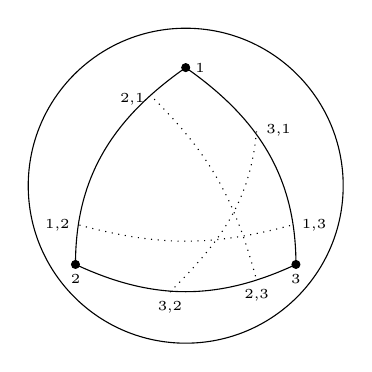
\begin{tikzpicture}
  \draw (2,2) circle [radius=2];

  \draw (0.6, 1) to [out=-25, in=205]
  (3.4, 1) to [out=90, in=-35]
  (2, 3.5) to [out=215, in=90]
  (0.6, 1);
  \draw[fill] (2, 3.5) circle [radius=0.05] node[anchor=west] {\tiny 1};
  \draw[fill] (0.6, 1) circle [radius=0.05] node[anchor=north] {\tiny 2};
  \draw[fill] (3.4, 1) circle [radius=0.05] node[anchor=north] {\tiny 3};
  \draw[dotted] (0.65, 1.5)  node[anchor=east] {\tiny 1,2}
  to [out=-15, in=195] (3.35, 1.5) node[anchor=west] {\tiny 1,3};

  \draw[dotted] (1.8, 0.65) node[anchor=north] {\tiny 3,2}
  to [out=45, in=265] (2.9, 2.7) node[anchor=west] {\tiny 3,1};
  \draw[dotted] (1.6, 3.1) node[anchor=east] {\tiny 2,1}
  to [out=-45, in=105] (2.9, 0.8) node[anchor=north] {\tiny 2,3};
\end{tikzpicture}
\caption{Intersection of great circle arcs inside a spherical triangle,
and the small spherical triangle formed by the arcs. Exaggerated so that the
small triangle is visible; not to scale.}
\label{fig:intlines}
\end{figure}
This is Method 2 in geodesic dome terminology. Recall in our earlier discussion
of barycentric coordinates that on a plane triangle, we can draw a line
corresponding to each $\beta_i$, and those three lines meet at a point. On the
sphere, if we make the same construction, the lines do not meet at a point
(except on the edges), but instead intersect to form a small spherical
triangle. Take a point within that triangle as $\mathbf v$.
Typically the centroid is used, as it's easy to calculate,
although we'll discuss another variation.

(If there were any ambiguities, we used the program \texttt{geodesic}
from Antiprism\cite{antiprism} as a reference implementation.)

In analytic terms, use Slerp to determine the points on each triangle edge.
Take the cross product of the opposing pairs of points to determine the normal
to the intersecting plane corresponding to each line. Take the cross product of
each pair of normals to find a vector proportional to the point of
intersection. (As the cross product is antisymmetric, be careful about order
here.) Then normalize each vector and take their centroid.

In terms of equations, Method 2 or the Great Circle Intersection
method on a triangle is:
\begin{equation}\begin{split}%??? does this reduce to slerp on the edges?
\mathbf v^* & = \sum^3_{i=1} \frac{\mathbf h_i \times \mathbf h_{i+1}}
{\|\mathbf h_i \times \mathbf h_{i+1}\|} \\
\mathbf h_i & =
\mathrm{Slerp}(\mathbf v_{i-1}, \mathbf v_i; \beta_{i})
\times
\mathrm{Slerp}(\mathbf v_{i+1}, \mathbf v_i; \beta_{i})
\end{split}\end{equation}

The above equation can be tweaked slightly by removing the step of normalizing
the vectors at the points of intersection. This still produces a point within
the triangle. This formula is a little more computationally efficient and
easier to treat algebraically. Where $\mathbf h_i$ is as before:
\begin{equation}\label{eq:gct}%??? does this reduce to slerp on the edges?
\mathbf v^* = \sum^3_{i=1} \mathbf h_i \times \mathbf h_{i+1} \\
\end{equation}

This method can be extended to the Quadrilateral. Use Slerp to find points on
opposing sides of the quadrilateral, use the cross product to find their
normal, and then use the cross product to find the point of intersection. Since
we draw two intersecting lines, there is only one point of intersection within
the quadrilateral. The formula is:
\begin{equation}\label{eq:gcq}%??? does this reduce to slerp on the edges?
\mathbf v^* =
(\mathrm{Slerp}(\mathbf v_1, \mathbf v_2; \frac{x+1}{2})
\times
\mathrm{Slerp}(\mathbf v_4, \mathbf v_3; \frac{y+1}{2}))
\times
(\mathrm{Slerp}(\mathbf v_1, \mathbf v_4; \frac{y+1}{2})
\times
\mathrm{Slerp}(\mathbf v_2, \mathbf v_3; \frac{x+1}{2}))
\end{equation}

\subsection{Nested Slerp}
This is similar to the Great Circle method, except instead of using the great
circles to calculate the intersections of the lines, we use another spherical
linear interpolation to get a point near the intersection. We effectively use
the Lerp formulas from the section on coordinates, substituting Slerp for Lerp.
Unlike Lerp, Slerp does not commute, so we take the different permutations of
the arguments and combine the different points that result.

Triangular:
\begin{equation}\label{eq:nst}
\mathbf v^* = \sum^3_{i=3} \mathrm{Slerp}(
\mathrm{Slerp}(\mathbf v_{i-1}, \mathbf v_i; \beta_{i}),
\mathrm{Slerp}(\mathbf v_{i+1}, \mathbf v_i; \beta_{i});
\frac{\beta_{i-1}}{1-\beta{i}})
\end{equation}
Quadrilateral:%??? not symmetric?
\begin{equation}\label{eq:nsq}
  \begin{split}
\mathbf v^* =& \mathrm{Slerp}(
\mathrm{Slerp}(\mathbf v_1, \mathbf v_2; \frac{x+1}{2}),
\mathrm{Slerp}(\mathbf v_4, \mathbf v_3; \frac{x+1}{2}); \frac{y+1}{2})\\
&+ \mathrm{Slerp}(
\mathrm{Slerp}(\mathbf v_1, \mathbf v_4; \frac{y+1}{2}),
\mathrm{Slerp}(\mathbf v_2, \mathbf v_3; \frac{y+1}{2}); \frac{x+1}{2})
\end{split}
\end{equation}

\subsection{Naive Slerp}
The previously mentioned mappings are all somewhat complicated. Expansion of the
formulas results in very lengthy equations. Applying a simplifying restriction
allows us to produce a formula that is nearly as simple as the gnomonic mapping.
The restriction is that the polygons are equilateral. This may seem very
restrictive, but many of the applications of these mappings involve a regular
polyhedron, e.g. the cube or the icosahedron, with equilateral faces.

The Naive Slerp method resembles a naive extension of spherical linear
interpolation (Slerp) to barycentric or $uv$ coordinates, thus the
name. Let $\cos(w) = \mathbf v_i \cdot \mathbf v_{i+1}$ for all $i$. (As
usual, the subscripts loop around.) For triangles:
\begin{equation}
   \mathbf v^* = \sum_{i=1}^3\frac{\sin(w\beta_i)}{\sin(w)}  \mathbf v_i
\end{equation}
For quadrilaterals:
\begin{equation}\begin{split}
     \mathbf v^* & = \sum_{i=1}^4\frac{\sin(w\gamma_i)}{\sin(w)} \mathbf v_i \\
\gamma_1 & = \frac{(1-x)(1-y)}{4} \\
\gamma_2 & = \frac{(1+x)(1-y)}{4} \\
\gamma_3 & = \frac{(1+x)(1+y)}{4} \\
\gamma_4 & = \frac{(1-x)(1+y)}{4}
\end{split}\end{equation}
or
\begin{equation}\begin{split}
   \mathbf v^* & = \sum_{i=1}^4\frac{s_i}{\sin^2(w)}  \mathbf v_i \\
s_1 & = \sin \left(w\frac{1-x}{2}\right)\sin \left(w\frac{1-y}{2}\right) \\
s_2 & = \sin \left(w\frac{1+x}{2}\right)\sin \left(w\frac{1-y}{2}\right) \\
s_3 & = \sin \left(w\frac{1+x}{2}\right)\sin \left(w\frac{1+y}{2}\right) \\
s_4 & = \sin \left(w\frac{1-x}{2}\right)\sin \left(w\frac{1+y}{2}\right) \\
\end{split}\end{equation}

\subsection{Projection of $\mathbf v^*$}
The nested slerp and naive slerp methods produce values that are normalized
along the edges. Because the projected edges already lie on the sphere, we have
freedom in how to adjust $\mathbf v^*$ to lie on the sphere. The easiest is
just to centrally project the vertices, that is, to normalize $\mathbf v^*$
like we have been. Another option is to perform a parallel projection along the
face normal, as defined earlier. We need the parallel distance $p$ from the
vertex to the sphere surface in the direction of the face normal
$\hat{\mathbf n}$, such that $\hat{\mathbf v} =
\mathbf v^* + p\hat{\mathbf n}$. $p$ is given by:
\begin{equation}
   p = -\mathbf v^* \cdot \hat{\mathbf n} +
   \sqrt{1+\mathbf v^* \cdot \hat{\mathbf n}-\mathbf v^* \cdot \mathbf v^*}
\end{equation}
$p$ can also be approximated as $\widetilde{p} = 1 - \|\mathbf v^*\|
\leq p$, which is fewer operations and doesn't require
calculation of the face normal. Technically, you can project in almost any
direction, not just that of the face normal, but most other choices don't
produce a symmetric result.

Sometimes the best mapping comes from a compromise of the central and
parallel projections. Choose a constant $k$, typically between 0 and 1, then:
\begin{equation}
  \hat{\mathbf v} = \frac{\mathbf v^* + kp\mathbf c}{\|\dots\|}
\end{equation}
$p$ may be replaced by $\widetilde{p}$. If our goal is to optimize a
measurement of the mapping, we can do a 1-variable optimization on $k$.

\section{Mappings between Euclidean polygons and disks}
Some of the mappings mentioned above adapt nicely to maps between regular
Euclidan polygons and disks in the Euclidean plane. Mappings between squares
and disks are well-represented in the literature, but mappings between
triangles and disks have been neglected.
\cite{fong15}\cite{fong16}\cite{fong18}\cite{lambers}

In this section, we will use a square with vertices
\begin{equation}
  \mathbf{v}_1 = \frac{[-1,-1]}{\sqrt 2}, \,
  \mathbf{v}_2 = \frac{[1,-1]}{\sqrt 2}, \,
  \mathbf{v}_3 = \frac{[1,1]}{\sqrt 2}, \,
  \mathbf{v}_4 = \frac{[-1,1]}{\sqrt 2},
\end{equation}
and a triangle with vertices
\begin{equation}
  \mathbf{v}_1 = \left[1, 0\right], \,
  \mathbf{v}_2 = \left[-\frac{1}{2}, \frac{\sqrt{3}}{2}\right], \,
  \mathbf{v}_3 = \left[-\frac{1}{2}, -\frac{\sqrt{3}}{2}\right].
\end{equation}
$[u, v]$ designates the point on the disk.

The mappings in this section can be adapted into mappings between a polygon and
a hemisphere. The stereographic projection conformally maps
the unit disk to a hemisphere, and is given by:
\begin{equation}\begin{split}
  \hat{\mathbf v} &= \frac{[2x, 2y, x^2+y^2-1]}{1+x^2+y^2}, \\
  [x, y] & = \frac{[v_x, v_y]}{1-v_z}.
\end{split}\end{equation}
The orthographic projection also maps the disk to the hemisphere,
and is given by:
\begin{equation}
  \hat{\mathbf v} = [x, y, \sqrt{1-x^2-y^2}].
\end{equation}

\subsection{Conformal}
\begin{equation}
f(z) = \int_0^z \prod_{k=1}^n (\zeta - z_k)^{\alpha_k-1} d\zeta
\end{equation}
 Like the Schwarz triangle map above,
computing this integral usually results in a hypergeometric function,
which is not particularly convenient. For squares it results in an elliptic
function, which is slightly more convenient.\cite{fong16}

\subsection{Radial stretching}
Consider the disk in polar coordinates. These mappings only change the radius
$r$ by a multiple, and leave $theta$ the same. They are not smooth. We give
only the triangular and square mappings here, but radial stretching is
extensible to any polygon. The square mapping is given in \cite{fong15} as:
\begin{equation}
  [u, v] = \frac{\max(|x|,|y|)}{\sqrt{x^2+y^2}} [x,y]
\end{equation}
The triangular mapping is somewhat easier to express in polar form:
\begin{equation}\begin{split}
  r &= 1-3 \min( \beta_i ) \\
  \theta &= \arctan\left(\sqrt{3}(\beta_2-\beta_3),
  3\beta_1 - 1 \right)
\end{split}\end{equation}
which can be converted back into Cartesian coordinates if needed.

\subsection{Naive Slerp}

Quadrilateral:
\begin{equation}\begin{split}
u &= \sqrt 2 \left(\sqrt{2+\sqrt 2} \sin \left( \frac{\pi}{8} x \right)
\cos \left( \frac{\pi}{8} y \right) \cos \left( \frac{\pi}{8} xy \right)
- \sqrt{2-\sqrt 2} \cos \left( \frac{\pi}{8} x \right) \sin
\left( \frac{\pi}{8} y \right) \sin \left( \frac{\pi}{8} xy \right)\right), \\
v &= \sqrt 2 \left(\sqrt{2+\sqrt 2} \cos \left( \frac{\pi}{8} x \right)
\sin \left( \frac{\pi}{8} y \right) \cos \left( \frac{\pi}{8} xy \right)
- \sqrt{2-\sqrt 2} \sin \left( \frac{\pi}{8} x \right)
\cos \left( \frac{\pi}{8} y \right) \sin \left( \frac{\pi}{8} xy \right)\right)
\end{split}\end{equation}
2nd Quadrilateral:
\begin{equation}\begin{split}
u &= \sqrt 2
\sin \left(\frac{\pi}{4}x\right) \cos \left(\frac{\pi}{4}y\right),\\
v &= \sqrt 2 \cos \left(\frac{\pi}{4}x\right) \sin \left(\frac{\pi}{4}y\right)
\end{split}\end{equation}
Note that the 2nd Quadrilateral Naive Slerp map preserves diagonal lines.

Triangular:
\begin{equation}\begin{split}
u& =  \frac{1}{\sqrt{3}} \left(2 \sin\left(\frac{2\pi}{3} \beta_1 \right)
- \sin\left(\frac{2\pi}{3} \beta_2 \right)
- \sin\left(\frac{2\pi}{3} \beta_3 \right) \right)\\
v& = \sin\left(\frac{2\pi}{3} \beta_2 \right)
- \sin\left(\frac{2\pi}{3} \beta_3 \right)
\end{split}
\end{equation}

\section{Applications}
\subsection{Cartographic use}

\subsection{Optimization of geodesic polyhedra}

\bibliographystyle{plain}
\bibliography{references}

\end{document}
